%%%%%%%%%%%%%%%%%%%%%%%%%%%%%%%%%%%%%%%%%
% Beamer Presentation
% LaTeX Template
% Version 1.0 (10/11/12)
%
% This template has been downloaded from:
% http://www.LaTeXTemplates.com
%
% License:
% CC BY-NC-SA 3.0 (http://creativecommons.org/licenses/by-nc-sa/3.0/)
%
%%%%%%%%%%%%%%%%%%%%%%%%%%%%%%%%%%%%%%%%%

%----------------------------------------------------------------------------------------
%	PACKAGES AND THEMES
%----------------------------------------------------------------------------------------

\documentclass{beamer}

\mode<presentation> {

% The Beamer class comes with a number of default slide themes
% which change the colors and layouts of slides. Below this is a list
% of all the themes, uncomment each in turn to see what they look like.

%\usetheme{default}
%\usetheme{AnnArbor}
%\usetheme{Antibes}
%\usetheme{Bergen}
%\usetheme{Berkeley}
%\usetheme{Berlin}
%\usetheme{Boadilla}
\usetheme{CambridgeUS}
%\usetheme{Copenhagen}
%\usetheme{Darmstadt}
%\usetheme{Dresden}
%\usetheme{Frankfurt}
%\usetheme{Goettingen}
%\usetheme{Hannover}
%\usetheme{Ilmenau}
%\usetheme{JuanLesPins}
%\usetheme{Luebeck}
%\usetheme{Madrid}
%\usetheme{Malmoe}
%\usetheme{Marburg}
%\usetheme{Montpellier}
%\usetheme{PaloAlto}
%\usetheme{Pittsburgh}
%\usetheme{Rochester}
%\usetheme{Singapore}
%\usetheme{Szeged}
%\usetheme{Warsaw}

% As well as themes, the Beamer class has a number of color themes
% for any slide theme. Uncomment each of these in turn to see how it
% changes the colors of your current slide theme.

%\usecolortheme{albatross}
%\usecolortheme{beaver}
%\usecolortheme{beetle}
%\usecolortheme{crane}
%\usecolortheme{dolphin}
%\usecolortheme{dove}
%\usecolortheme{fly}
%\usecolortheme{lily}
%\usecolortheme{orchid}
%\usecolortheme{rose}
%\usecolortheme{seagull}
%\usecolortheme{seahorse}
%\usecolortheme{whale}
%\usecolortheme{wolverine}

%\setbeamertemplate{footline} % To remove the footer line in all slides uncomment this line
%\setbeamertemplate{footline}[page number] % To replace the footer line in all slides with a simple slide count uncomment this line

%\setbeamertemplate{navigation symbols}{} % To remove the navigation symbols from the bottom of all slides uncomment this line
}

\usepackage{graphicx} % Allows including images
\usepackage{booktabs} % Allows the use of \toprule, \midrule and \bottomrule in tables
\usepackage{multicol}
\usepackage{subcaption}

\AtBeginSection{\frame{\sectionpage}}

%----------------------------------------------------------------------------------------
%	TITLE PAGE
%----------------------------------------------------------------------------------------

\title[COMP 5411 Rendering Project]{Rendering Thin Film Interference on Soap Bubbles} % The short title appears at the bottom of every slide, the full title is only on the title page

\author{Mucong Ding} % Your name
\institute[HKUST] % Your institution as it will appear on the bottom of every slide, may be shorthand to save space
{
Hong Kong University of Science and Technology \\ % Your institution for the title page
\medskip
\textit{mcding@connect.ust.hk} % Your email address
}
\date{\today} % Date, can be changed to a custom date

\begin{document}

\begin{frame}
\titlepage % Print the title page as the first slide
\end{frame}

\begin{frame}
\frametitle{Overview} % Table of contents slide, comment this block out to remove it
\begin{multicols}{2}
	\tableofcontents
\end{multicols} % Throughout your presentation, if you choose to use \section{} and \subsection{} commands, these will automatically be printed on this slide as an overview of your presentation
\end{frame}

%----------------------------------------------------------------------------------------
%	PRESENTATION SLIDES
%----------------------------------------------------------------------------------------

%------------------------------------------------
\section{Background Theory}
%------------------------------------------------

\subsection{Introduction}

\begin{frame}
	\frametitle{Introduction (I)}
	What should be a soap bubble look like?
	\begin{figure}
	\centering
	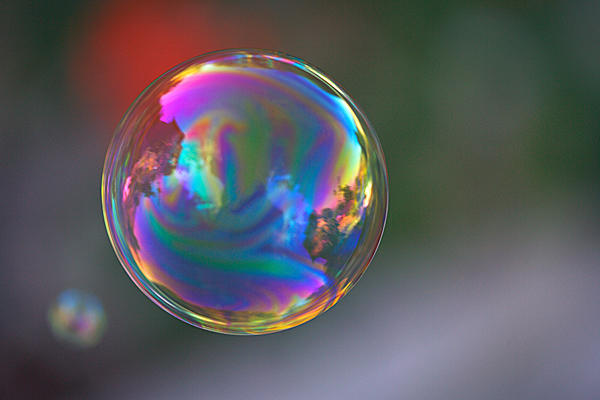
\includegraphics[width=0.5\linewidth]{real_world_bubble.jpg}
	\caption{A Real World Soap Bubble}
	\end{figure}
\end{frame}

%------------------------------------------------

\begin{frame}
	\frametitle{Introduction (II)}
	\begin{figure}
		\centering
		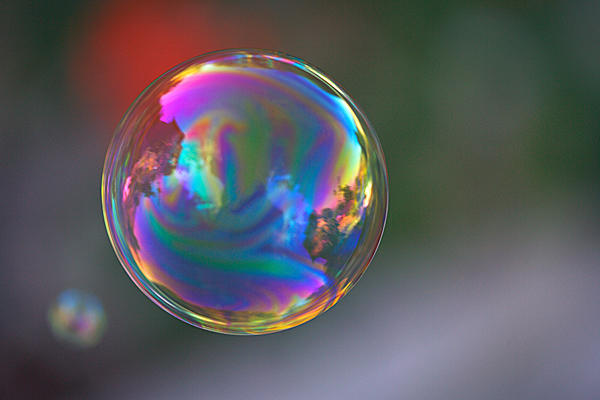
\includegraphics[width=0.3\linewidth]{real_world_bubble.jpg}
		\caption{A Real World Soap Bubble}
	\end{figure}
	There are three dominant effects
	\begin{itemize}
		\item Reflection 
		\item Refraction with high Fresnel Effect
		\item Thin film interference (colors)
	\end{itemize}
	The third effect is usually omitted by CG simulation.
\end{frame}

%------------------------------------------------

\begin{frame}
	\frametitle{Introduction (III)}
	How to simulate thin film interference?
	\begin{itemize}
		\item Go deeper in physics
		\item Design workable approximated shading algorithm
	\end{itemize}
\end{frame}

%------------------------------------------------

\subsection{Physics Background}

\begin{frame}
	\frametitle{Fresnel Equation}
	The well-know Fresnel shader in CG is designed based on the Fresnel Equation.
	\begin{itemize}
		\item $R_{\textrm{S}} = \frac{n_1 \cos\theta - n_2\sqrt{1 - (\frac{n_1}{n_2}\sin\theta)^2}}{n_1 \cos\theta + n_2\sqrt{1 - (\frac{n_1}{n_2}\sin\theta)^2}}$
		\item $R_{\textrm{P}} = \frac{n_1\sqrt{1 - (\frac{n_1}{n_2}\sin\theta)^2} - n_2 \cos\theta}{n_1\sqrt{1 - (\frac{n_1}{n_2}\sin\theta)^2} + n_2 \cos\theta}$
		\item Reflectance as function of refractive indices ratio $n_1/n_2$ and incident angle $\theta$
		\item Polarization matters, \textrm{S} and \textrm{P} polarization components of lights
	\end{itemize}
\end{frame}

%------------------------------------------------

\begin{frame}
	\frametitle{Thin Film Effect}
	Thin film: two very close interfaces with thickness $d \sim 1000$ nm.
	\begin{itemize}
		\item Refracted light cancel or reinforce depends on the thickness-to-wavelength ratio $d/\lambda$
		\item Approximate effective reflectance derived by applying Fresnel equation twice
		\item $	R(\lambda, \theta, d) = 2R_{\textrm{P}}^2\frac{1-\cos\delta}{1+R_{\textrm{P}}^4-2R_{\textrm{P}}^2\cos\delta}+2R_{\textrm{S}}^2\frac{1-\cos\delta}{1+R_{\textrm{S}}^4-2R_{\textrm{S}}^2\cos\delta}$
		\item $ \delta(\lambda, \theta, d) = 4\pi n\frac{d}{\lambda}\cos\theta $
		\item Ignore polarization (by averaging) since when don't have enough information
	\end{itemize}
	\begin{figure}
	\centering
	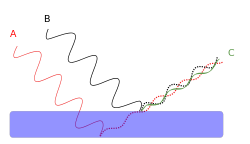
\includegraphics[width=0.3\linewidth]{thin_film_theory.png}
	\caption{Thin Film Interference}
	\end{figure}
\end{frame}

%------------------------------------------------

\subsection{The Shading Equation}

\begin{frame}
	\frametitle{The Shading Equation}
	Idea: Effective reflection and transmission as if only one interface:
	\begin{itemize}
		\item $	L_P(\lambda) = (1-R(\lambda, \theta, d))L_{it}(\lambda) + R(\lambda, \theta, d)L_{ir}(\lambda) $
		\item Reflectance $R(\lambda, \theta, d)$ defined on the previous slide
		\item Wave-length $\lambda$ matters!
	\end{itemize}
\end{frame}

%------------------------------------------------
\section{The Shaders}
%------------------------------------------------

\subsection{Color and Wavelength}

\begin{frame}
	\frametitle{Color and Wavelength}
	The shading equation depends on wave-length $\lambda$, how can we obtain it?
	\begin{itemize}
	\item Assigning approximate wave-lengths to each of the RGB components
	\item R $\sim 660$ nm, G $\sim 510$ nm, B $\sim 450$ nm
	\item Treat them differently from start to end
	\item Code:
	\end{itemize}
	\begin{figure}
	\centering
	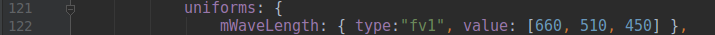
\includegraphics[width=1.00\linewidth]{color_code.png}
	\end{figure}
	\begin{figure}
	\centering
	
\includegraphics[width=0.7\linewidth]{color_wavelength.png}
	\caption{Spectral Colors}
	\end{figure}
\end{frame}

%------------------------------------------------

\subsection{Thickness Distribution}

\begin{frame}
	\frametitle{Thickness Distribution}
	Uniform thickness $d$ on the surface is not physical, makes interference colors only appears when incident angles is close to $90$ deg.\\
	Simulate the thickness distribution on the globe!\\
	Two main effects
	\begin{itemize}
		\item Drifting: by gravity
		\item Sloshing: by perturbation
	\end{itemize}
	\begin{figure}
    \centering
	\begin{subfigure}[b]{0.2\textwidth}
		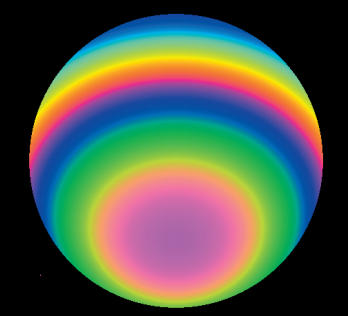
\includegraphics[width=\textwidth]{thickness_drifting.png}
		\caption{\footnotesize Only Drifting}
	\end{subfigure}
	\quad\quad
	\begin{subfigure}[b]{0.2\textwidth}
		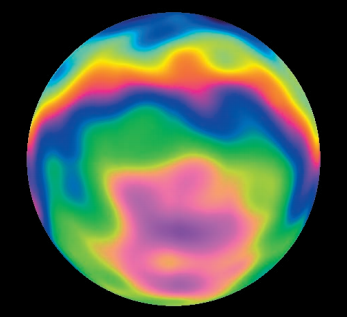
\includegraphics[width=\textwidth]{thickness_sloshing.png}
		\caption{\footnotesize Add Sloshing}
	\end{subfigure}
	\end{figure}
	Code:
	\begin{figure}
		\centering
		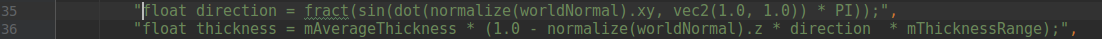
\includegraphics[width=1.0\linewidth]{thickness_code.png}
	\end{figure}
\end{frame}

%------------------------------------------------

\subsection{Following the Physics}

\begin{frame}
	\frametitle{Following the Physics (I)}
	The major part of shaders following the physics equations.\\
	Vertex Shader:
	\begin{figure}
		\centering
		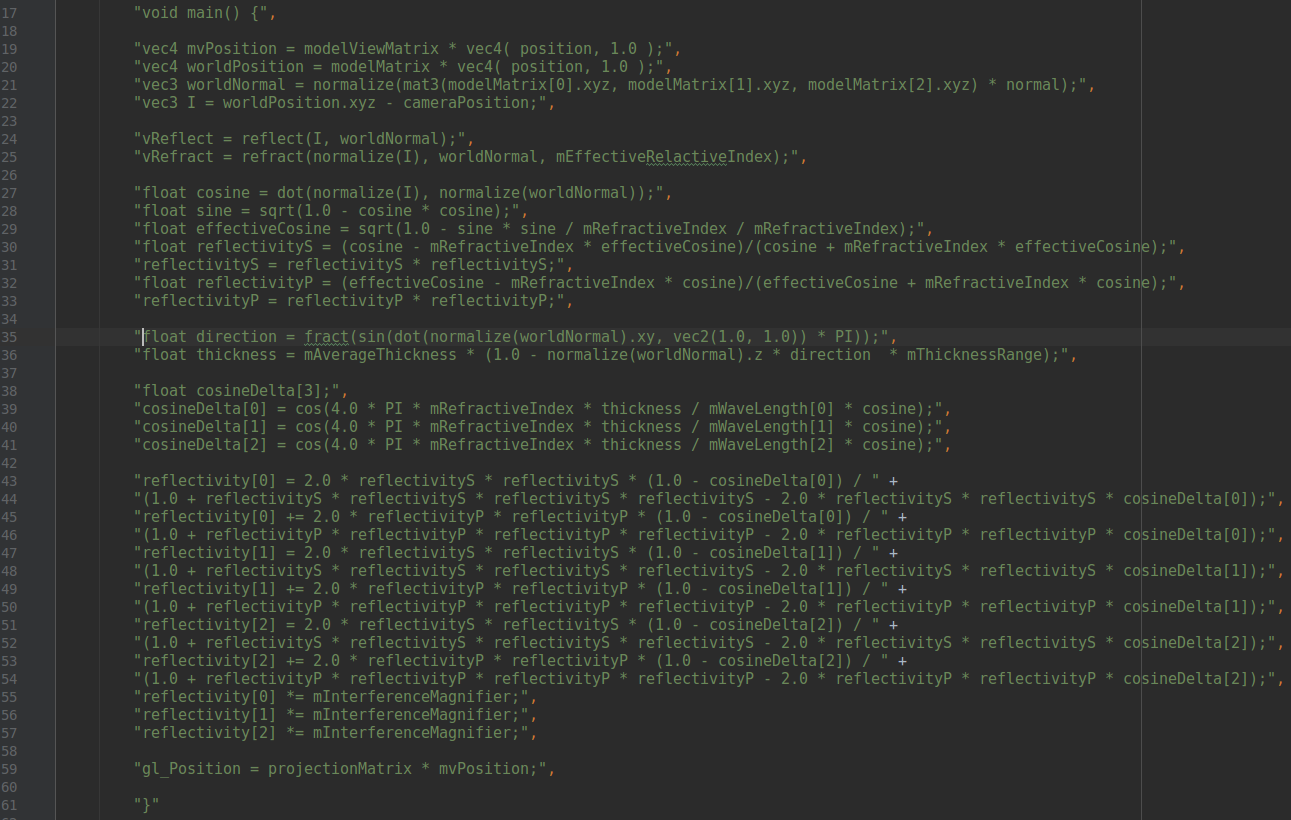
\includegraphics[width=0.8\linewidth]{vertex_shader.png}
	\end{figure}
\end{frame}

%------------------------------------------------

\begin{frame}
	\frametitle{Following the Physics (II)}
	Fragment Shader:
	\begin{figure}
		\centering
		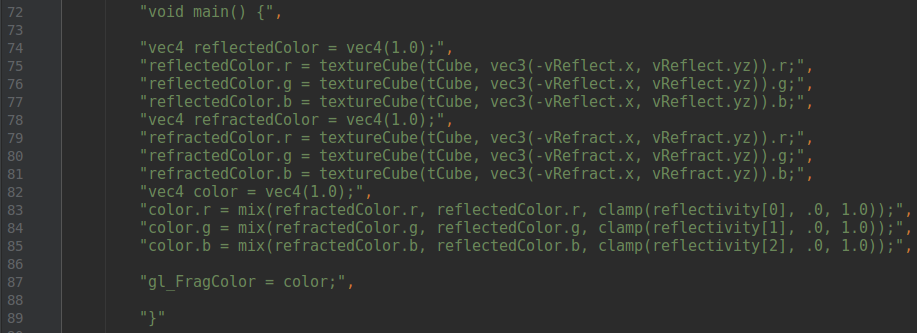
\includegraphics[width=0.8\linewidth]{fragment_shader.png}
	\end{figure}
\end{frame}

%------------------------------------------------
\section{Live Demo}
%------------------------------------------------

\subsection{Demonstration}

\begin{frame}
	\frametitle{Demonstration}
	Demo first!
	\begin{itemize}
		\item \url{http://mcding.student.ust.hk/comp5411/}
	\end{itemize}
\end{frame}

%------------------------------------------------

\subsection{Summary of Observations}

\begin{frame}
	\frametitle{Summary of Observations}
	What we have:
	\begin{itemize}
		\item Colors! (thin film interference)
		\item Fresnel effect originated from Fresnel equation itself!
	\end{itemize}
	What we don't have:
	\begin{itemize}
		\item Only texture mapping, no good light sources (may magnify interference and Fresnel effects)
		\item Good simulation of transmission through the bubble (4 interfaces) (approximated by an effective refractive index $ n_e \sim 1.005 $ now)
	\end{itemize}
\end{frame}

%------------------------------------------------
\section{Challenges, Result, and Future Work}
%------------------------------------------------

\subsection{Challenges and Result}

\begin{frame}
	\frametitle{Challenges and Result}
	Challenges:
	\begin{itemize}
	\item Deriving approximated shading equation from real physics (partially aided by reference [2])
	\item Assigning RGB components with different wave-lengths to simulate compound color light
	\item Simulating drifting and sloshing which affect thickness distribution
	\item Dynamic texture mapping and setting up the scene (with the help of skeleton example [1])
	\end{itemize}
	Result:
	All challenges solved.
\end{frame}

%------------------------------------------------

\subsection{Future Work and Reference}

\begin{frame}
	\frametitle{Future Work and Reference}
	Future Work:
	\begin{itemize}
		\item Adding light source
		\item Ray tracing
		\item Distortion matters
	\end{itemize}
	Reference:
	\begin{figure}
		\centering
		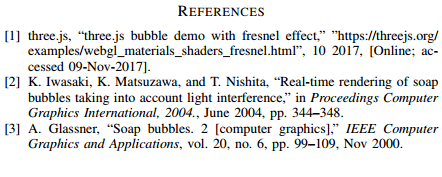
\includegraphics[width=0.8\linewidth]{reference.png}
	\end{figure}
\end{frame}

%------------------------------------------------

\end{document}